\chapter{Realisierung des Source-To-Source Compilers}
\label{chap:Realisierung}
Gestützt auf das grundsätzliche Wissen über Compiler, die herausgearbeiteten Unterscheidungen von  Xamarin.Forms und Flutter sowie die Differenzen der verwendeten Programmiersprachen  \Csharp{} und Dart, wird in diesem Kapitel die Realisierung des Source-to-Source Compilers beschrieben.  Es bietet sich die \ac{ide} (deutsch Entwicklungsumgebung) Visual Studio 2019 von Microsoft an,  um das Projekt mit Roslyn Integration zu implementieren,  da auf dieser Plattform Erweiterungen für Roslyn zur Verfügung stehen.
Die zu entwickelnde Projektmappe besteht also aus dem Source-to-Source Compiler mit Roslyn-Integration, der grafischen Benutzeroberfläche und einer Xamarin.Forms Anwendung als Testobjekt,  wobei letztere jedoch erst im nächsten Kapitel thematisiert wird.


\section{Programmablauf}
Mithilfe des Roslyn Compilers kann der Source-to-Source Compiler Auswertungen zu den in der Xamarin.Forms App referenzierten Quelltextdateien durchführen.  Somit ist es möglich,  eine Auflistung aller verfügbaren \Csharp-Dateien aus einem Projekt zu extrahieren.  XAML-Dateien werden nicht von Roslyn behandelt.  Dies gelingt jedoch über den Umweg der Codebehind-Dateien mit Endung .XAML.cs,  die ein Laden über das Dateisystem ermöglichen. 

Bevor der Source-to-Source Compiler alle Quelltext- und Ansichtsdateien übersetzt,  müssen die in Kapitel 4 beschriebenen Metadaten überführt werden.  Anschließend kann der Quelltext optimiert und der Übersetzungsvorgang abgeschlossen werden.  Zur Visualisierung des Übersetzungsvorganges dient das in Abbildung \ref{fig:umlablauf} dargestellte \ac{uml}-Aktivitätsdiagramm.

\newpage
\begin{figure}[!ht]
 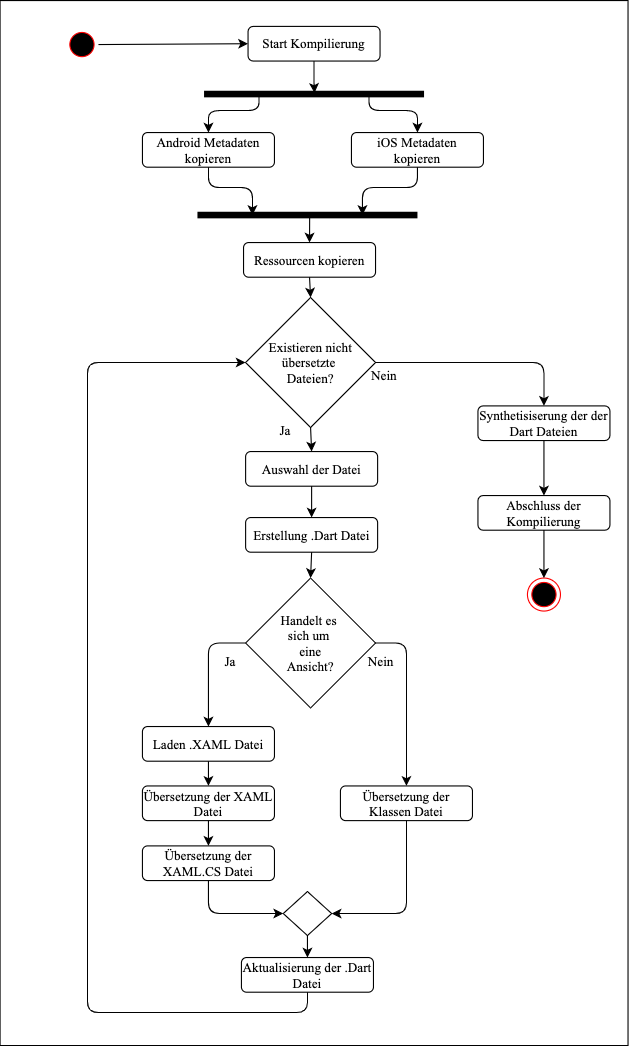
\includegraphics[width=\textwidth,keepaspectratio]{Images/Implementation/Ablauf.png}
 \caption{Compiler-Ablauf als UML Aktivitätsdiagramm}
 \label{fig:umlablauf}
\end{figure}

Das dargestellte \ac{uml}-Diagramm befindet sich aufgrund der Komplexität des Compilers auf einer hohen Abstraktionsebene. In den folgenden Abschnitten werden die einzelnen Aspekte der Kompilierung noch näher betrachtet.


\section{Metadaten}
Wie das UML Diagramm veranschaulicht, können die Metadaten von Android und iOS parallel in die Flutter Anwendung kopiert werden.  Da die Metadaten
plattformspezifische Eigenschaften der mobilen Anwendungen sind, wird im nächsten Abschnitt auf die entsprechenden Details der beiden Betriebssysteme eingegangen.


\subsection{Android Metadaten}
Zu den Android spezifischen Metadaten gehören die sogenannten Launcher Icons, die den Anwendern als App-Icon angezeigt werden. Xamarin.Android speichert diese grafischen Symbole in Ordnern, die die unterschiedlichen Pixeldichten der Android-Geräte unterstützen und in denen unter Umständen auch andere Bilder gespeichert sind.  Innerhalb von Xamarin.Forms wird das ausgewählte Icon über die Klasse  \glq MainActivity.cs\grq{}  definiert, wie in Quelltext \ref{lst:IconName} dargestellt. 

\lstinputlisting[label={lst:IconName},caption={Xamarin.Forms Android Launcher-Icon Name}, language=csh]{SourceCode/IconName.cs}

Nach der Extraktion des Namens können die entsprechenden Bilder kopiert werden.  In der durch die Flutter SDK erzeugten App liegen bereits Bildplatzhalter für den Austausch bereit.

Der eindeutige Identifizierer,  PackageID,  zählt ebenfalls zu den Metadaten und dient der unverwechselbaren Erkennung einer Anwendung auf dem mobilen Gerät und im Google Play Store.  Die Information über die PackageID kann in Xamarin.Forms aus der \glq AndroidManifest.xml\grq{} Datei ausgelesen werden und muss in Flutter sowohl in drei Manifest Dateien als auch in die \glq build.gradle\grq{} Konfiguration geschrieben werden.  Das Plugin \glq change\_app\_package\_name\grq{}  nimmt alle notwendigen Änderungen vor.  Es ist als Abhängigkeit zum Projekt hinzuzufügen und anschließend über die Kommandozeile auszuführen. 

Der Anwendungsname wird, wie die PackageID,  aus dem AppManifest extrahiert und in Flutter allerdings nur in eine Manifest Datei im Verzeichnis \glq Project/app/src/main\grq{} geschrieben.  Die Berechtigungen,  die während der Laufzeit der Anwendung beantragt werden,  befinden sich ebenfalls innerhalb des AppManifests und können von hier kopiert werden.

\subsection{iOS Metadaten}
Xamarin.iOS verwaltet die für die Übersetzung notwendigen Metadaten in einer Datei im  Projektverzeichnis mit dem Namen \glq Info.plist\grq .  In Flutter Apps gibt es eine entsprechende Datei,  jedoch werden die Inhalte,  beispielsweise die Bildnummer und der Identifizierer,  aus Variablen geladen.  Damit nach der Kompilierung kein erhöhter Administrationsaufwand bei der Verwaltung dieser Eigenschaften entsteht,  soll dieses Schema beibehalten werden.  Die \glq AppFrameworkInfo.plist\grq{} stellt die Quelle aller Werte,  die als Variablen in die \glq Info.plist\grq, geladen werden müssen dar.   Daher werden die entsprechenden Einträge aus der \glq Info.plist\grq{} von Xamarin.Forms extrahiert und jeweils in die entsprechenden \glq Info.plist\grq{} Dateien von Flutter kopiert.  Tabelle \ref{tab:InfoPlist} zeigt die Zieldatei für die Kopie bestimmter Werte.

\begin{table}[!ht]
  \begin{tabularx}{\linewidth}{|l|X|X|}
  \hline

  \textbf{Schlüssel}  &  \textbf{Info.plist} & \textbf{AppFrameworkInfo.plist} \\
\hline
  DevelopmentRegion  		&  					& 		\checkmark	 \\
  ShortVersionString  		&  					& 		\checkmark	 \\
  Version  							&  					& 		\checkmark	 \\
  MinimumOSVersion  		&  					& 		\checkmark	 \\
  
  InterfaceOrientations  		& \checkmark  	&		 					\\
  BundleSignature  			&  \checkmark 	& 							\\
  BundleName  					&  \checkmark 	& 		 					\\
  \hline
\end{tabularx}
\caption{Einträge in \glq Info.plist\grq-Dateien in Flutter}
 \label{tab:InfoPlist}
\end{table}
Die Übersicht weist nicht alle aus der iOS Entwicklung bekannten Schlüssel auf.  Alle fehlenden Eigenschaften gehören in die Datei \glq Info.plist\grq, wie die letzten drei in der Tabelle \ref{tab:InfoPlist} genannten.  Ähnlich dem Vorgehen bei den Android Metadaten kann für die Modifizierung  von Anwendungsnamen und Identifizierer auf iOS eine Erweiterung verwendet werden.  So kann der Compiler das \glq rename\grq{} Plugin verwenden und es bedarf keiner zusätzlichen manuellen Entwicklung. \footcite[Vgl.][Abgerufen am \today]{Rename}  Die aus iOS bekannten Texte,  zur Beantragung von Berechtigungen müssen weiterhin vom Source-To-Source Compiler extrahiert und in die Flutter \glq info.plist\grq{} transferiert werden.

Für das Anwendungsicon kann das Verzeichnis \glq Assets.xcassets\grq{} aus dem Stammverzeichnis der Xamarin.Forms iOS App in das Verzeichnis \glq ios/flutter/Runner\grq , das alle notwendigen Bilder enthält,  kopiert werden. 

\section{Ressourcen}

Neben den Metadaten ist die Ressourcenkopie der mobilen Anwendung vonnöten.  Dazu gehören die innerhalb der App angezeigten Bilder, die bei Xamarin.Forms üblicherweise innerhalb der plattformspezifischen Anwendungen abgelegt sind. Von dort aus kopiert der Compiler die Bilder aus dem iOS Projekt in das Flutter Projekt zur späteren Verwendung.  Da für Bilder im Flutter Framework keine plattformspezifische Unterscheidung vorgesehen ist,  werden ausschließlich die Bilder aus der iOS App entnommen.  Eine Entscheidung zugunsten der iOS Alternativen wurde  getroffen,  da sich die Konzepte von Xamarin.iOS und Flutter im Bezug auf Bilderressourcen ähneln und eine automatisierte Überführung möglich ist.  Android spezifische Varianten werden während der Übersetzung also nicht berücksichtigt.   
Zur Speicherung und Darstellung höher aufgelöster Bilder existieren zwei Unterordner mit den Namen  \glq 2.0x\grq{} und  \glq 3.0x\grq{} im Verzeichnis Assets.  Ressourcen werden je nach Skalierungsfaktor  \glq @2x\grq{} oder  \glq @3x\grq{} in den entsprechenden Verzeichnissen und ohne Option im Ordner Asset abgelegt.
Neben dem differenzierten Vorgehen bei der Kopie ist es erforderlich,  die Ressourcen in der \glq pubspec.yaml\grq{} zu referenzieren.  Ein Ausschnitt aus der \glq pubspec.yaml\grq ,  der das Einbinden von Bildern demonstriert,  wird in Quelltext \ref{lst:RefImage} dargestellt.

\lstinputlisting[label={lst:RefImage},caption={Referenzierung von Bildern in der pubspec.yaml}, language=Dart]{SourceCode/FlutterPubspecImage.pub} 


Benutzerdefinierte Schriftsätze müssen ebenfalls aus dem iOS Verzeichnis kopiert und anschließend in der \glq pubspec.yaml\grq Datei hinzugefügt werden.  Hier gilt,  analog zu den Bildern,  dass die kompilierte Flutter Anwendung ausschließlich die Schrift der iOS App verwendet und androidspezifische Schriftsätze verloren gehen.

Weitere Ressourcen bilden die Startbildschirme der verschiedenen Plattformen,  die während des Ladens der App angezeigt werden und für eine Veröffentlichung im Appstore verpflichtend sind.  Durch ihren simplen Aufbau entsteht keine zusätzliche Ladezeit und ihr Quelltext wird plattformspezifisch realisiert.  Der Compiler verarbeitet ausschließlich einzelne Bilder, die während des Ladens der mobilen Anwendung angezeigt werden und verzichtet auf die Übersetzung des plattformspezischen Programmcodes,  wie in den Ausschlusskriterien erwähnt.  Da die Xamarin.Forms App nicht zwangsläufig ein Bild in einem entsprechenden Format vorhält,  greift der Flutter Startbildschirm auf das LauncherIcon der jeweiligen Plattformen zurück.  

\section{Übersetzung von Klassenstrukturen}

Die Übersetzung von \Csharp{} zu Dart ist ein essentieller Bestandteil des Compilers.  Dafür wird zuerst die Visual Studio Projektmappe geladen.  Anschließend kann fokussiert das Projekt betrachtet werden, welches den plattformunabhängigen Quelltext beinhaltet.  Da dieser selbst, wie bereits in den Ausschlusskriterien erwähnt,  unübersetzt bleibt, sind die entsprechenden Projekte ausschließlich für das Kopieren der Metadaten und Ressourcen notwendig.  Alle Klasse durchlaufen die in Quelltext \ref{lst:CsharpFrontend} dargestellten Ausführungsschritte. 
\lstinputlisting[label={lst:CsharpFrontend},caption={C\# Compiler Frontend}, language=csh]{SourceCode/CompilerFrontEnd.cs}
Für die Übersetzung von einer Programmiersprache zu einer anderen ist es notwendig,  alle Knoten und Token innerhalb eines Syntaxbaums in der richtigen Reihenfolge zu betrachten.  Die abstrakte Klasse \glq CSharpSyntaxWalker\grq{} erlaubt es,  einen eigenen \glq Syntax-Walker\grq{} zu konstruieren,  der die Knoten und Token analysiert.  Dafür kann von \glq CSharpSyntaxWalker\grq{} geerbt und folgend die \glq Visit()\grq{} Methode überschrieben werden.  \footcite[Vgl.][Abgerufen am \today]{Varty2014}  Der Quelltext \ref{lst:CsharpFrontend} visualisiert die Erstellung eines \glq FlutterTranspilerVisitors\grq ,  mithilfe des vorher ermittelten semantischen Models.  Nun wird der ausgelesene Wurzelknoten des Syntaxbaumes als Parameter der \glq Run()\grq{} Methode übergeben,  die den \glq Visitor\grq{} startet.  

Hiermit endet das Compiler Frontend und es beginnt die Konstruktion des Dart Programmcodes.  Dafür werden die einzelnen Knoten des Baumes je nach ihrem Typen zu entsprechenden Dart Synonymen umgewandelt und die einzelnen Methoden des \glq CSharpSyntaxVisitor\grq{} überschrieben.  Quelltext \ref{lst:PropertyDeclaration} zeigt die Umwandlung von Eigenschaftsdeklarationen.
\newpage
\lstinputlisting[label={lst:PropertyDeclaration},caption={Compilierung von Eigenschaftsdeklarationen}, language=csh]{SourceCode/Modifizierer.cs}

Der Quelltextausschnitt veranschaulicht die generelle Arbeitsweise des Compilers,  der einzelne Zeichen und Zeilen des Dart-Textdokumentes generiert und speichert.  So hangelt sich der Compiler durch das Dokument und übersetzt den Quelltext Schritt für Schritt, wobei die Reihenfolge, in der der Typ, der Zugriffsmodifizierer und der Name der Eigenschaft in die Dart Datei geschrieben wird,  von entscheidender Bedeutung ist.  Die Quelltextzeilen 6 bis 8 geben zuerst den Eigenschaftstyp,  gefolgt von dem optionalen Zugriffsmodifizierer und dem Namen aus.  Zusätzlich kann nun ein Wert gesetzt werden,  bevor ein Semikolon die Deklaration beendet.  Die Methode für die Generierung des Dart Modifizierers zeigt Quelltext \ref{lst:DartModifier}.


\lstinputlisting[label={lst:DartModifier},caption={Austausch von C\# Zugriffsmodifizierern}, language=csh]{SourceCode/Modifier.cs}

Wie bereits in Kapitel 5 beschrieben,  sind die Typen der beiden Programmiersprachen nicht identisch und müssen daher entsprechend angepasst werden.  Zur Veranschaulichung wird die realisierte Methode in Quelltext \ref{lst:DataType} dargestellt. 
\lstinputlisting[label={lst:DataType},caption={Austausch von C\# Datentypen}, language=csh]{SourceCode/Datatypes.cs}

Der Rückgabewert dieser Methode ist der entsprechende Dart Datentyp.  Sollte keine entsprechende Repräsentation verfügbar sein,  erfolgt die Rückgabe des ursprünglichen Typnamens.  Dies ist notwendig,  um andere übersetzte Klassen im Quelltext verwenden zu können.  Damit keine unerwünschten Typen des .Net Frameworks oder von Xamarin.Forms Erweiterungen innerhalb des Übersetzungsergebnisses erscheinen, sind Bereinigungen erforderlich. 

Erweiterungen ergänzen die Funktionalität der Frameworks,  sind jedoch herstellerabhängig mit unterschiedlichen Anforderungen programmiert,  sodass es für Klassen und Methoden aus diesen Bibliotheken nicht zwangsläufig identische Repräsentationen gibt.  Eine Auflösung der Inkompatibilität ist nicht mittels Automation möglich, sondern bedarf unterschiedlich umfangreicher manueller Umwandlungen.  Der Komplexität ist es geschuldet,  dass der Compiler nur eine Auswahl von Erweiterungen unterstützt.  Nachträgliche Erweiterungen des Funktionsumfanges sind möglich.  Die folgenden Anwendungsfälle skizzieren das Vorgehen.  

Mobile Anwendungen nutzen Bilder, die neu über die Kamera aufgenommen werden oder aus der bestehenden Galerie stammen.  Im folgenden wird der Quelltext dargestellt, der die Funktionalität des Xamarin.Forms Essentials mit dem Flutter Plugin \glq image\_picker\grq{} austauscht.  Die notwendigen Berechtigungen wurden bereits während der Übernahme der Metadaten gesetzt und können daher an dieser Stelle ignoriert werden.

\lstinputlisting[label={lst:MediaPlugin},caption={Austausch der Kamera und Galerie Erweiterung}, language=csh]{SourceCode/ImagePluginSwap.cs}

Ein weiterer wichtiger Anwendungsfall,  der nur durch Erweiterungen implementiert werden kann,  ist der Zugriff auf die Smartphone Sensoren.  Der folgende Quelltext zeigt den Austausch der Beschleunigungssensorfunktionen des Xamarin.Essentials Plugins mithilfe des Flutter Sensor Plugins.  Der Compiler übersetzt ebenfalls die Funktionalität des Gyroskops, siehe Programmcode \ref{lst:Sensor}. Da der Quelltext jedoch analog ist, wird er an dieser Stelle nicht explizit aufgeführt. 

\lstinputlisting[label={lst:Sensor},caption={Austausch der Beschleunigungssensor Erweiterung}, language=csh]{SourceCode/Accelerometer.cs}

 Obwohl es keine Gewährleistung gibt, dass für jede Xamarin Forms eine entsprechende Flutter 
Erweiterung zur Verfügung steht, konnte bei der Implementierung des Compilers immer eine  Alternative gefunden werden.


\section{Übersetzung von Ansichten}
Xamarin.Forms Ansichten bestehen, wie bereits beschrieben,  aus den XAML und XAML.CS Dateien, die nach der jeweiligen Übersetzung  in einer gemeinsamen Dart Datei synthetisiert werden.  
Die Kompilierung der beiden Dateien geschieht jeweils durch ein dediziertes Compiler Frontend, das die Aufgaben bis zur Zwischendarstellung übernimmt.  Darauf aufbauend wird ein gemeinsames Compiler-Backend für die Zusammenführung und die Code-Optimierung entwickelt.  Die Abbildung  \ref{fig:ViewCompilerPhases} veranschaulicht den Vorgang. 

\begin{figure}[!ht]
 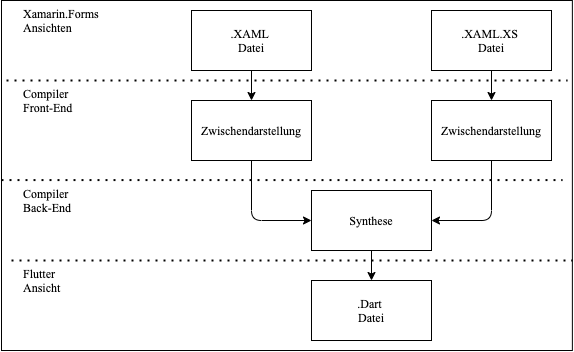
\includegraphics[width=\textwidth,keepaspectratio]{Images/Implementation/ViewCompiler.png}
 \caption{Compiler-Phasen für die Übersetzung von Ansichten}
 \label{fig:ViewCompilerPhases}
\end{figure}

\subsection{Visuelle- Zwischendarstellung}

Für die visuelle Zwischendarstellung wird in einem ersten Schritt die XML Struktur
aus der XAML Datei ausgelesen und als Syntaxbaum interpretiert.  Er beinhaltet eine Auflistung von untergeordneten Elementen,  die weitere Elemente beinhalten können,  sodass eine Verschachtelung  entsteht.  Jedes Element besitzt eine Auflistung von Eigenschaften, die Attribute der einzelnen XML Knoten beschreiben.  Die baumartige Struktur des Xamarin.Forms Layouts wird durch die in Kapitel 4 beschriebenen Repräsentationen von Flutter Widgets in einen Flutter Widget-Baum überführt und für jedes Widget der Quelltext zur Initialisierung in einem Template vorgehalten.  Alle Eigenschaften besitzen in dieser Vorlage vorgefertigte Platzhalter, wie in Quelltext \ref{lst:Placeholder} dargestellt.

\lstinputlisting[label={lst:Placeholder},caption={Vorlage eines Flutter Text-Widgets} , language=Dart]{SourceCode/DartPlaceholder.dart} 

Aufgrund von Inkompatibilitäten zwischen den von Xamarin.Forms gelieferten und von Flutter erwarteten Eigenschaftswerten, ist es notwendig diese umzuwandeln.  Der folgende Quelltext \ref{lst:Parsing} zeigt die Modifizierung von Textgrößen.  Xamarin.Forms fordert den Wert entweder als Zahl oder als sogenannte benannte Größe,  wie \glq Large\grq{} oder \glq Title\grq , während Flutter ausschließlich Textgrößen mit dem Typen Double akzeptiert.   

\lstinputlisting[label={lst:Parsing},caption={Umwandlung von Schriftgrößen} , language=csh]{SourceCode/CSharpFontSize.cs} 

Mittels vergleichbarer Implementierung sind auch an anderen Eigenschaften,  wie z.B. Farbwahl oder Textumbruchoptionen,  Anpassungen erforderlich.

Nun erfolgt die Anlage einer Arbeitskopie des Templates,  um in weiteren Compilerphasen die Werte aus der Xamarin.Forms App einzufügen.  Abbildung \ref{fig:PlaceholderOptions} visualisiert die Behandlung der Platzhalter in den einzelnen Phasen der Übersetzung.


\begin{figure}[!ht]
 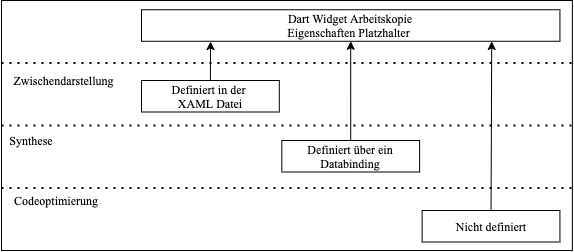
\includegraphics[width=\textwidth,keepaspectratio]{Images/Implementation/DartPlaceHolder.png}
 \caption{Bereinigung von Platzhaltern}
 \label{fig:PlaceholderOptions}
\end{figure}

Es wird deutlich, dass in der Zwischendarstellung ausschließlich XAML definierte Eigenschaftswerte 
importiert werden.  Während der Synthese erfolgt der Austausch der sogenannten Databindings, die den Wert aus der Codebehind-Datei erhalten.  Zur Übersetzung werden neue Platzhalter mit dem Prefix \glq BindingPlaceholder\grq{} benötigt,  die in der Arbeitskopie hinterlegt sein müssen. Exemplarisch wird in Quelltext  \ref{lst:PlaceholderBinding} der Text-Platzhalter zu einem Binding Platzhalter umgewandelt, und der Platzhalter textAlign mit einem Wert versehen. 

\lstinputlisting[label={lst:PlaceholderBinding},caption={Flutter Widget mit Binding-Platzhaltern} , language=Dart]{SourceCode/DartPlaceholderBinding.dart} 

Zu diesem Zeitpunkt sind in der Arbeitskopie noch die Binding- und die ungenutzten Platzhalter vorhanden.  Diese müssen, wie in der Abbildung \ref{fig:PlaceholderOptions} visualisiert,  in späteren Phasen der Kompilierung entfernt werden.  Grundsätzlich lässt sich aus der XAML Datei ableiten,  welche Platzhalter nicht benötigt werden.  Da die Bereinigung jedoch eine Teilaufgabe der Optimierung darstellt, wird sie erst in der entsprechenden Phase im Compiler-Backend durchgeführt. 

\subsection{Logische Zwischendarstellung}

Die Erzeugung der logischen Zwischendarstellung,  basierend auf den Codebehind Dateien,  erfordert die gleiche Implementierung mit \glq CSharpSyntaxWalker\grq{} wie die der Klassenstrukturen,  da es sich bei diesen Dateien ebenfalls um \Csharp{} Klassen handelt.  

Xamarin.Forms übermittelt Änderungen an  Eigenschaften automatisch, mithilfe der \glq INotifyPropertyChanged\grq{}  Schnittstelle, an die Benutzeroberfläche.  Bei Flutter erhält das Framework durch die \glq setState\grq{}  Methode entsprechende Informationen.  Der Compiler kann notwendige Änderungen erst im Backend und nicht im Rahmen der Zwischendarstellung durchführen,  da anhand der Codebehind Dateien nicht identifizierbar ist, welche Eigenschaften einen direkten Bezug auf die graphische Benutzeroberfläche haben. 

\subsection{Visuelle Synthese}

Die Zusammenführung der visuellen und logischen Zwischendarstellung erfolgt während der visuellen Synthese im Compiler-Backend.  In einem ersten Schritt erfolgt die Kopie der übersetzten Logik unterhalb der für den Aufbau der grafischen Benutzeroberfläche beinhalteten \glq Build\grq{} Methode.  Im nächsten Schritt werden ereignisauslösende Aktivitäten,  beispielsweise der Klick auf Schaltflächen wie in Quelltext \ref{lst:Synth} dargestellt,  mit den übersetzten Methoden verbunden und die Platzhalter entfernt.  Dabei wird der Name der behandelten Methode aus der XML Struktur extrahiert und der entsprechende Binding-Platzhalter mit dem Namen und dem Parameter \glq Context\grq{} ersetzt. 


\lstinputlisting[label={lst:Synth},caption={Synthese von ereignisauslösenden Aktivitäten} , language=csh]{SourceCode/ClickSynth.cs} 

Die Sicherstellung der automatischen Aktualisierung der Benutzeroberfläche kann an dieser Stelle durch die Verwendung von SetState-Blöcken realisiert werden.  Dafür wird der Eigenschaftsname aus dem Binding-Platzhalter extrahiert und im Quelltext überprüft, wo die entsprechende Eigenschaft manipuliert wird.  Die ermittelten Zeilen werden anschließend mit einem SetState-Block eingeschlossen.


\section{Referenzierung}
Im Anschluss an die Zwischendarstellung, in der die Generierung von Logik und Ansichten erfolgte,  müssen nun die entstandenen Dartartefakte untereinander referenziert werden.  Darunter wird in diesem Zusammenhang die Verknüpfung der entsprechenden Quelltextdokumente verstanden.  Diese Verlinkung ist erforderlich,  damit Komponenten auf Klassen zugreifen können,  die in anderen Dateien definiert sind.  Im Gegensatz zu \Csharp{} können Dateien in Dart nicht über Namespaces, sondern nur über ihren Dateinamen eingebunden werden.  Folglich ist es erforderlich,  Dateien in Quelltextdokumente einzubinden,  die verwendete Klassendefinition enthalten.  Die Information,  in welcher Datei sich eine Klasse befindet, wird durch den \glq CSharpSyntaxWalker\grq{} festgehalten.  Diese Referenzen werden ebenfalls benötigt,  um durch die Anwendung zu den Navigationszielen zu gelangen, da es sich bei der Navigation um die Erzeugung eines Objektes des entsprechenden Widgets handelt. 


\section{Codeoptimierung}

Nach der erfolgreichen Zusammenführung der einzelnen Artefakte kann der Code optimiert werden. Dafür werden Sprachkomponenten einschließlich der Ereignisdefinition,  der Ereignishandler und aller Aufrufe entfernt, die  nur für die  Arbeit von Xamarin.Forms benötigt  wurden. Die Löschung betrifft die \glq InitializeComponent\grq{}  Methode, die aus der Codebehind-Datei die grafische Benutzeroberfläche geladen hat und die bereits durch SetState-Blöcke ersetzte
 \glq INotifyPropertyChanged\grq{}  Schnittstellendefinition,  die für die Oberflächenaktualisierung zuständig war.  Jetzt folgt die Entfernung der nicht benötigten Platzhalter mit dem in Quelltext \ref{lst:PlaceholderCleanup} dargestellten Algorithmus,  aus dem generierten Dart Quelltext.  
\lstinputlisting[label={lst:PlaceholderCleanup},caption={Bereinigung von ungenutzten Platzhaltern}, language=csh]{SourceCode/Cleanup.cs}
Damit befindet sich der Programmcode in einem korrekten syntaktischen Zustand und kann mithilfe des Flutter Compilers zu einer mobilen App übersetzt und ausgeführt werden.  Ein zusätzlicher Schritt der Codeoptimierung verbessert die Lesbarkeit des erzeugten Quelltextes durch eine einheitliche Formatierung. Der mit Templates generierte Widget-Baum ist innerhalb der Build Methode nicht eingerückt. Zur Bereinigung bietet die Flutter-SDK die Möglichkeit,  Quelltextdokumente über die Kommandozeilenschnittstelle zu formatieren.  Quelltext \ref{lst:Formatting} zeigt die Methode zur Quelltextformatierung durch die SDK. 

\lstinputlisting[label={lst:Formatting},caption={Methode zur Quelltextformatierung} , language=csh]{SourceCode/FlutterFormatting.cs} 


\section{Grafische Benutzeroberfläche}
Die \ac{gui} ist der zentrale Berührungspunkt von Anwendern mit dem Transpiler.  Sie soll die notwendigen Eingabemöglichkeiten anbieten, das Ergebnis ausgeben und den Anwender auf mögliche Fehler hinweisen.  Das grafische Vorbild ist das in Kapitel 3 entworfene Mockup, siehe Abbildung 3.4.  Für die Erstellung einer entsprechenden Benutzeroberfläche stehen eine Vielzahl von Technologien mit verschiedenen Vor- und Nachteilen zur Verfügung.  Eine Webseite erspart dem Anwender einen hohen Installationsaufwand und ermöglicht die plattformunabhängige Verwendung des Compilers.  Allerdings ist zumindest ein gewisser Kontrollverlust über den eigenen Quelltext durch das  Hochladen auf eine Webseite nicht ausgeschlossen.  Die Bedienoberfläche dieser Arbeit soll daher eine lokale Anwendung sein, sodass kein  unberechtigter Zugriff auf den Source-Code möglich ist.  Zu diesem Zweck wird die \ac{gui}  mit der Technologie \ac{wpf} realisiert.  Dabei handelt es sich um ein UI-Framework des .NET Frameworks, das für die Erstellung von mit XAML und \Csharp{} entwickelten Desktopanwendungen geeignet ist. \footcite[Vgl.][S. 1f]{Wenger2012} 

Anwendungen,  die mittels WPF programmiert werden, sind nur unter Windows als Betriebssystem ausführbar.  Da der Roslyn Compiler auch nur unter Windows verfügbar ist,  entstehen hier keine zusätzlichen Einschränkungen.  Die folgende Darstellung \ref{fig:CompilerUI} zeigt das Erscheinungsbild der Anwendung nach einer erfolgreichen Übersetzung.
\newpage
\begin{figure}[!ht]
 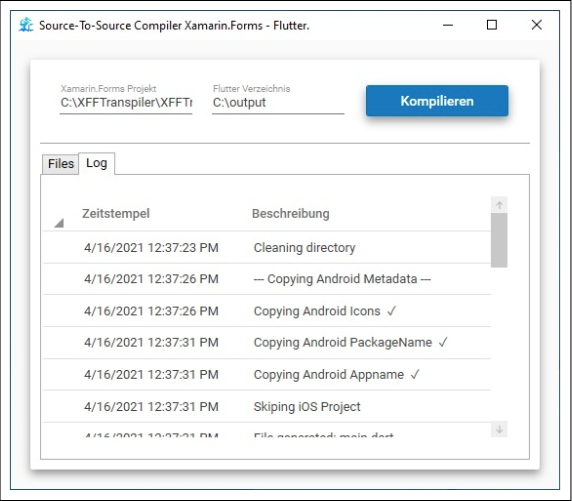
\includegraphics[width=\textwidth,keepaspectratio]{Images/Implementation/UiScreenshot.png}
 \caption{Grafische Oberfläche des Compilers}
 \label{fig:CompilerUI}
\end{figure}

Wie die Ansicht veranschaulicht, werden die durchgeführten Arbeitsschritte durch Log-Einträge in der Anwendung angezeigt.
Die Realisierung der grafischen Benutzeroberfläche 
und des Source-To-Source Compilers erfolgte mit  .Net Technologien,  sodass es möglich ist,  den Compiler als Abhängigkeit in das Projekt der grafischen Benutzeroberfläche zu laden und von dort aus die Übersetzung zu starten.  Eine vollständige Anleitung für die Installation der \ac{gui}  befindet sich in  \hyperref[chap:Installationsanleitung]{Anhang V}.